\chapter{Testy nowej metody}

W tym rozdziale zostaną przedstawione porównania opracowanej metody. W pierwszej kolejności zaprezentowane zostanie zestawienie z metodą wytrenowaną z wykorzystaniem paradygmatu end-to-end, a zatem explicite modelującą ocenę radiologa. Następnie przedstawione zostanie porównanie z wynikami prac algorytmu oceniającego proces gojenia się ścięgna Achillesa z wykorzystaniem danych z Ultrasonografii. Ostatnie zestawienie dotyczy porównania wyników z oceną biomechaniczną.

Zarówno metoda oparta o paradygmat end-to-end jak i o dane Ultrasonograficzne są wynikiem prac, w których autor tej rozprawy był współautorem, nadzorował grupę studentów opracowujących finalne rozwiązania oraz tworzył plan badań. W przypadku oceny biomechanicznej prace nad metodą zrealizowane zostały w całości przez mgr Magdalenę Syrek z Carolina Medical Center w Warszawie, zatem wartością dodaną tej rozprawy jest przedstawione porównanie.   

\section{Porównanie z metodą opartą o paradygmat end-to-end}
\label{seq:end-to-end}
W tej sekcji opracowana metoda zostanie porównana z metodą opartą o paradygmat end-to-end, modelującą explicite ocenę radiologa. Do tego zadania zostały wykorzystane trzy architektury sieci konwolucyjnych opisane w Rozdziale \ref{CNNs} tj. AlexNet, GoogLeNet (Inception-v3) i ResNet z 50 warstwami konwolucyjnymi (ResNet-50). Wszystkie trzy architektury zostały zmodyfikowane poprzez zastąpienie końcowej warstwy klasyfikacyjnej warstwą regresji z pojedynczym wyjściem i funkcją kosztu zdefiniowaną jako średni błąd kwadratowy. W skutek tego podejścia algorytm szkolony jest, aby minimalizować błąd pomiędzy predykcją sieci neuronowej, a wartościami parametrów z wzorca odniesienia. 

Do szkolenia się sieci wykorzystano powiększony zestaw treningowy, ograniczony jednak do danych z 44 pacjentów treningowych i trzech sekwencji wybranych w toku eksperymentów przedstawionych w podsekcji \ref{seq:protocol_selection}: T2 $^\ast$ GRE, T2 $^\ast$ GRE TE\_MIN i PD. Tym razem nie zdecydowano się na zawężenie zbioru danych tylko do jednej sekwencji RM z uwagi na potrzebę maksymalizację liczebności zbioru. Nie zdecydowano się również na pełny zbiór wszystkich sekwencji, z uwagi na różnice w danych, które mogłyby zaburzać proces szkolenia się. 

Do szkolenia zastosowano metodę kroswalidacji z podziałem na 4 segmenty. Dla każdego z parametrów z wzorca odniesienia wyszkolono osobną sieć. Wyliczono metryki MAE, MAX-AE i Corr stosowane również w poprzednim rozdziale. Wyniki zestawiono w Tab. \ref{tab:end-to-endTrain}.
\renewcommand{\arraystretch}{1.2}
\begin{table}[ht]
%\vspace{-px}
\scriptsize
\setlength{\tabcolsep}{1pt}
\centering
\caption{Wyniki szkolenia się sieci w paradygmacie end-to-end z wykorzystaniem zbioru treningowego. Pogrubieniem oznaczono najlepsze wyniki.}
\label{tab:end-to-endTrain}
\begin{tabular}{lc||c|c|c|c|c|c}
	%\hline
	&& \textbf{SCT} & \textbf{TT} & \textbf{STE} & \textbf{TE} & \textbf{TU} & \textbf{TisE}\\ \hline \hline
	AlexNet$_{e}$ & MAE & 1,04$\pm$0,33 & 0,82$\pm$0,27 & 0,95$\pm$0,48 & 0,88$\pm$0,38 & 1,03$\pm$0,36 & 0,78$\pm$0,26  \\
	&MAX-AE & 1,91 & 1,67 & 2,39 & 2,20 & 1,90 & 1,35\\ 
	&Corr & 0,82 & \textbf{0,72} & \textbf{0,13} & 0,70 & 0,50 & 0,83 \\ \hline
	Inception-v3$_{e}$ & MAE & 0,88$\pm$0,32 & \textbf{0,75}$\pm$0,22 & \textbf{0,82}$\pm$0,33 & \textbf{0,78}$\pm$0,20 & \textbf{0,91}$\pm$0,34 & \textbf{0,67}$\pm$0,23 \\
	&MAX-AE & 1,57 & \textbf{1,44} & \textbf{1,93} & \textbf{1,17} & \textbf{1,85} & \textbf{1,11} \\ 
	&Corr & \textbf{0,85} & \textbf{0,72} & 0,05 & \textbf{0,72} & \textbf{0,52} & \textbf{0,84} \\ \hline
	ResNet-50$_{e}$ & MAE & \textbf{0,64}$\pm$0,21 & 0,98$\pm$0,28 & 0,83$\pm$0,37 & 0,89$\pm$0,22 & 1,06$\pm$0,41 & 1,10$\pm$0,34  \\
	&MAX-AE & \textbf{1,21} & 1,79 & 1,94 & 1,43 & 2,42 & 2,36\\
	&Corr & 0,06 & 0,21 & 0,00 & 0,11 & 0,14 & 0,11\\
	
	
\end{tabular}
%\vspace{-0.5cm}
\end{table}
\renewcommand{\arraystretch}{1}

Otrzymane wartości MAE znajdują się w zakresie 0,64 do 1,10 (w skali wzorca odniesienia 0--7). Dla najlepszego modelu pod względem średniej MAE tj. Inception-v3, średni dystans między predykcją i wzorcem wyniósł $<0,92$. Najlepiej estymowanymi parametrami były TisE -- 0,67, TT -- 0,75 i TE -- 0,78. Najgorsze rezultaty natomiast otrzymano dla TU -- 0,91, który to parametr silnie zależy od informacji widocznej w płaszczyźnie strzałkowej.

W kolejnej tabeli (Tab. \ref{tab:end-to-end_testset}) przedstawiono zestawienie automatycznej oceny dla zbioru pacjentów testowych, realizowanej przez najlepszy model szkolony w paradygmacie end-to-end (IncepionV3) i proponowaną przez autora tej pracy metodą z meta-regresją opartą o algorytm SVR (SVR).  
\renewcommand{\arraystretch}{1.2}
\begin{table*}[t]
	\caption{Porównanie wyników wnioskowania z wykorzystaniem zbioru testowego dla metody proponowanej tj. SVR oraz metody wyszkolonej w paradygmacie end-to-end. Pogrubieniem oznaczono najlepsze wyniki.}
	\scriptsize
	\begin{center}
		\begin{tabular}{lc||c|c|c|c|c|c}
			\textbf{Model} & & \textbf{SCT} & \textbf{TT} & \textbf{STE} & \textbf{TE} & \textbf{TU} & \textbf{TisE}\\ \hline \hline
			Inception-v3$_{e}$ & MAE & 1,12$\pm{0,74}$ & 0,80$\pm{0,24}$ & 1,40$\pm{0,52}$ & \textbf{0,89}$\pm{0,31}$ & 1,08$\pm{0,26}$ & \textbf{0,69}$\pm{0,07}$ \\
			& MAX-AE & \textbf{2,14} & \textbf{1,01} & 2,13 & \textbf{1,18} & \textbf{1,44} & \textbf{0,78} \\
			& Corr & 0,82 & 0,77 & 0,05 & 0,59 & 0,02 & 0,77 \\ \hline
			SVR & MAE & \textbf{1,05}$\pm0,12$ & \textbf{0,56}$\pm0,06$ & \textbf{0,75}$\pm0,08$ & 0,91$\pm0,10$ & \textbf{0,91}$\pm0,09$ & $0,94\pm0,10$\\
			& MAX-AE & 2,62 & 1,82 & \textbf{1,92} & 2,54 & 2,01 & 2,38 \\
			& Corr & \textbf{0,85} & \textbf{0,85} & \textbf{0,31} & \textbf{0,72} & \textbf{0,65} & \textbf{0,80} 
		\end{tabular}
	\end{center}
	\label{tab:end-to-end_testset}
\end{table*}
\renewcommand{\arraystretch}{1}

Metoda SVR osiąga wyższe rezultaty Corr w każdym z parametrów i niższe MAE dla 4 z 6 parametrów. Natomiast tylko w jednym z parametrów (tj. STE) charakteryzuje się niższym MAX-AE. 

Można zatem wnioskować, że cechy wykorzystywane w metodzie SVR do oceny procesu gojenia się skuteczniej dywersyfikują kolejne fazy procesu i pozwalają na ocenę trendu z lepszą dokładnością niż metoda oparta o paradygmat end-to-end. 2 z 6 parametrów, w których pod względem MAE sieć Inception-v3$_e$ okazała się lepsza tj. TE i TisE dotyczą obrzęków, zatem elementów ocenianych pod kątem pola powierzchni i kształtu. Fakt ten należy interpretować, iż tego rodzaju informacja dominuje w ekstrahowanych przez jądra splotu obrazach, co z kolei implikuje gorsze wyniki w pozostałych parametrach ocenianych na podstawie wzorców tworzonych przez struktury ścięgniste. Wynik MAX-AE nie jest zaskakujący, ponieważ z uwagi na naturę treningu (explicite modelowanie wzorca odniesienia) maksymalne błędy będą minimalizowane. Trudność w interpretacji polega na fakcie, że maksymalne błędy mogą być wynikiem błędu algorytmu, jak również pojedynczymi omyłkami doświadczonego radiologa, który z uwagi np. na zmęczenie bądź inne dystrakcje zaburzające percepcję, popełnił błąd w ocenie.  

W tym kontekście należy również podkreślić zasadnicze różnice między dwoma przedstawionymi metodami. Do rozwoju metody end-to-end niezbędna jest pełna informacja od radiologa tj. ocena 6 parametrów w kolejnych krokach czasowych. Średnio jest to około 1 godziny pracy na pacjenta. Proponowana przez autora metoda wykorzystuje sieć wyszkoloną na bazie etykiet wyższego poziomu tj. rozróżniających jedynie oznaczenia zdrowych i chorych tkanek. Takie szkolenie jest nazywane słabo-nadzorowanym (w odróżnieniu od pełni-nadzorowanego w paradygmacie end-to-end). Dalszy rozwój proponowanej metody można zatem uzyskać przy wykorzystaniu danych oznaczonych jako chory, zdrowy oraz znacząco mniejszego zbioru pacjentów z oznaczonym pełnym wzorcem odniesienia, który posłużyłby do sporadycznych ulepszeń etapu meta-regresji. 

Pewnym minusem proponowanego podejścia jest wymóg informacji o ROI, jednakże jego oznaczenie to czas około 10 minut na pacjenta, dla radiologa wykorzystującego odpowiednie oprogramowanie np. Osirix \cite{Rosset2004} lub VisNow \cite{Nowinski_Borucki_2014}. Ponadto segmentację ROI można stosunkowo łatwo zautomatyzować. Wstępne prace dr. Jędrzeja Nowosielskiego i dr. Piotra Regulskiego oraz autora tej pracy pokazują, że skuteczne w tym zakresie mogą być sieci typu \textit{fully convolutional neural networks}. Przykład działania takiej architektury (tj. U-Net zaproponowanej w \cite{Ronneberger2015}) można zaobserwować na Rys. \ref{fig:segmentacja}. 

\begin{figure}[h]
	\centering
	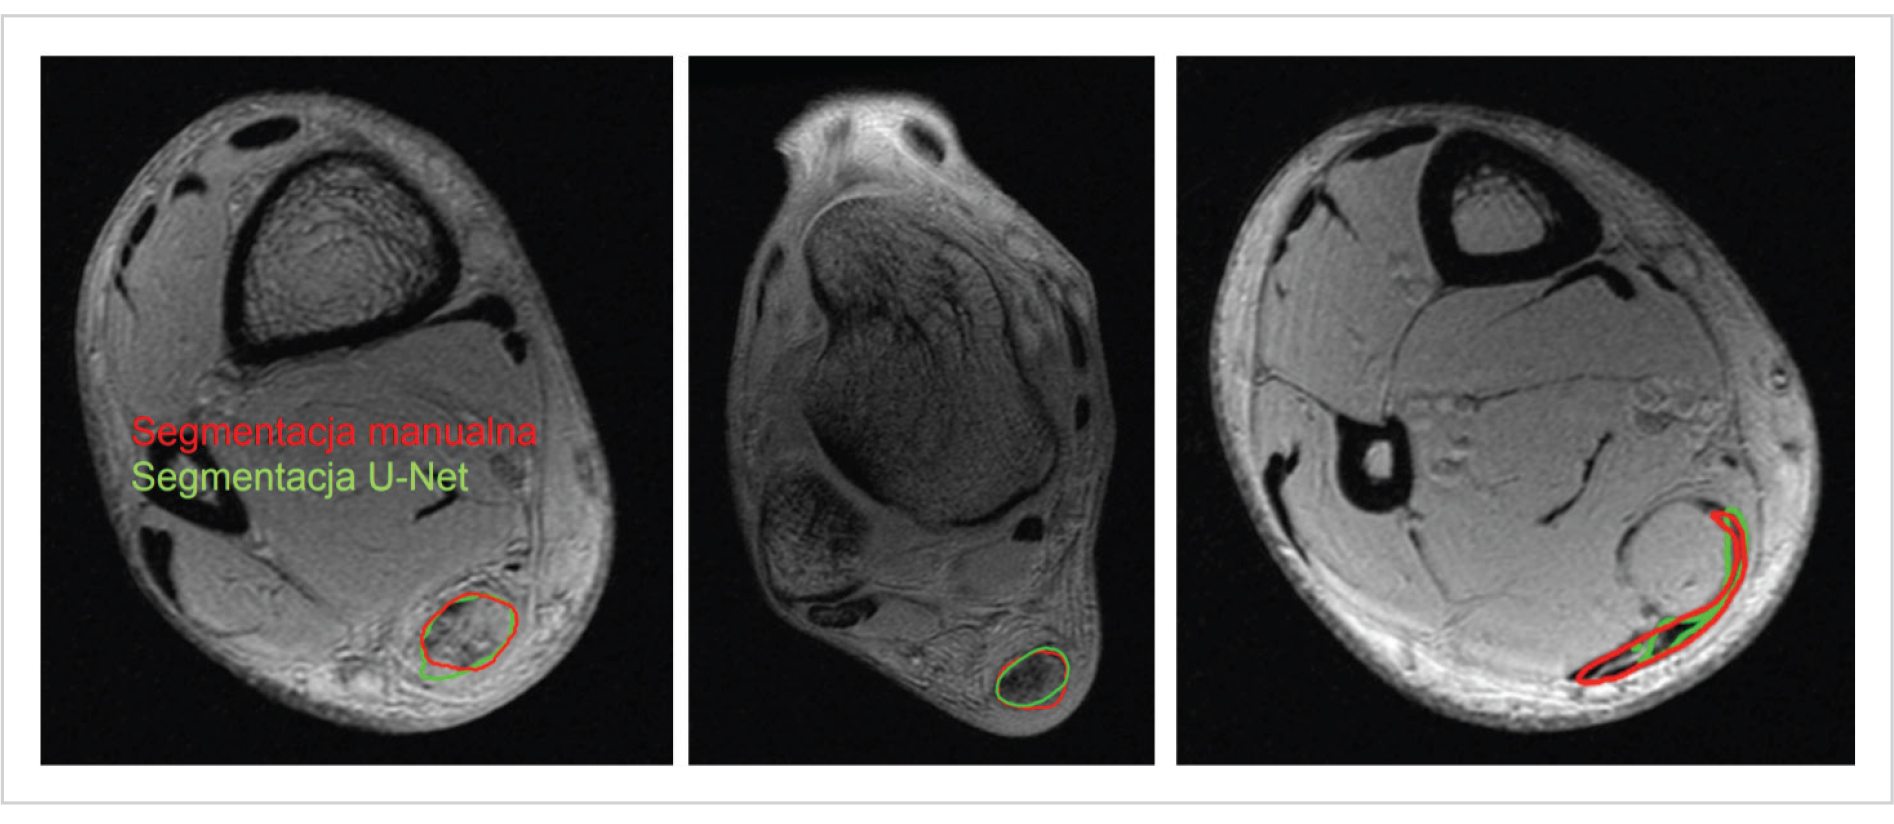
\includegraphics[width=1\textwidth]{figures/Segmentacja.jpg}
	\caption{Automatyczna segmantacja ROI z wykorzystaniem głębokich sieci neuronowych.}\label{fig:segmentacja}
\end{figure}
Kolorem czerwonym oznaczono obszar segmentacji manulanej, wykonanej przez eksperta radiologa. Kolorem zielonym efekt segmentacji automatycznej. Miara DICE (zob. \cite{Zou2004}) dla otrzymanych obrazów wynosi około 0.75 i świadczy o wysokiej jakości segmentacji oraz o obiecującym kierunku tego rodzaju prac.

Ciekawym elementem rozwoju automatycznej oceny byłaby również fuzja obu metod tj. podmiana ekstraktora cech DL trenowana na binarnie oznaczonym zbiorze na ekstraktor uzyskanego modelu Inception-v3. Jednak z uwagi na omawiane problemy praktyczne z dalszym rozwojem tak utworzonej metody oraz brak obiecujących rezultatów w przeprowadzonych przez autora tej pracy badaniach wstępnych, taka propozycja nie została uwzględniona w prezentowanej rozprawie. 

\section{Porównanie z metodą opartą o dane z ultrasonografii}
\label{seq:comp-usg}
W tej sekcji opracowana metoda została porównana z automatyczną oceną bazującą na danych z Ultrasonografii. Ponownie, do utworzenia metody opartej o USG wykorzystano konwolucyjne sieci neuronowe, a dokładniej AlexNet, Inception-v3 i ResNet-50 oraz wykorzystano omówiony w poprzedniej sekcji paradygmat end-to-end. 

Dane dla metody opartej o Ultrasonografię pochodziły również z projektu START. Stosowano się zatem do identycznych odstępów czasowych, co w przypadku badań RM, a akwizycji poddano tych samych pacjentów. Z przyczyn praktycznych zmniejszyła się jedynie grupa odniesienia, która w tym przypadku wyniosła 18-stu zdrowych ochotników. Badania zrealizowano z wykorzystaniem aparatu GE 3D high-resolution Voluson E8 Expert z liniową sondą (5--18 MHz). Jako dane wejściowe wykorzystano informacje z trybu B (zob. \ref{USG}), których ostateczna liczba wyniosła 565 skanów 3D. 

Dane USG są zbliżone do izotropowych dlatego utworzono zbiory zarówno w oparciu o przekroje w płaszczyźnie osiowej jak i strzałkowej (tylko tam, gdzie widoczne jest ścięgno):
\begin{itemize}
	\item zbiór treningowy USG (strzałkowy) -- zawiera 253.639 2D przekrojów w płaszczyźnie strzałkowej, w tym 245.366 pochodzących od chorych 44 pacjentów oznaczonych przez radiologa i 8.273 pochodzących od zdrowych ochotników.
	\item zbiór treningowy USG (osiowy) -- zawiera 467.548 2D przekrojów w płaszczyźnie osiowej, w tym 450.816 pochodzących od chorych 44 pacjentów oznaczonych przez radiologa i 16.732 pochodzących od zdrowych ochotników. 
\end{itemize}

Wizualizacja przykładowych danych USG znajduje się na Rys. \ref{fig:US_sample}.
\begin{figure}[h!]
	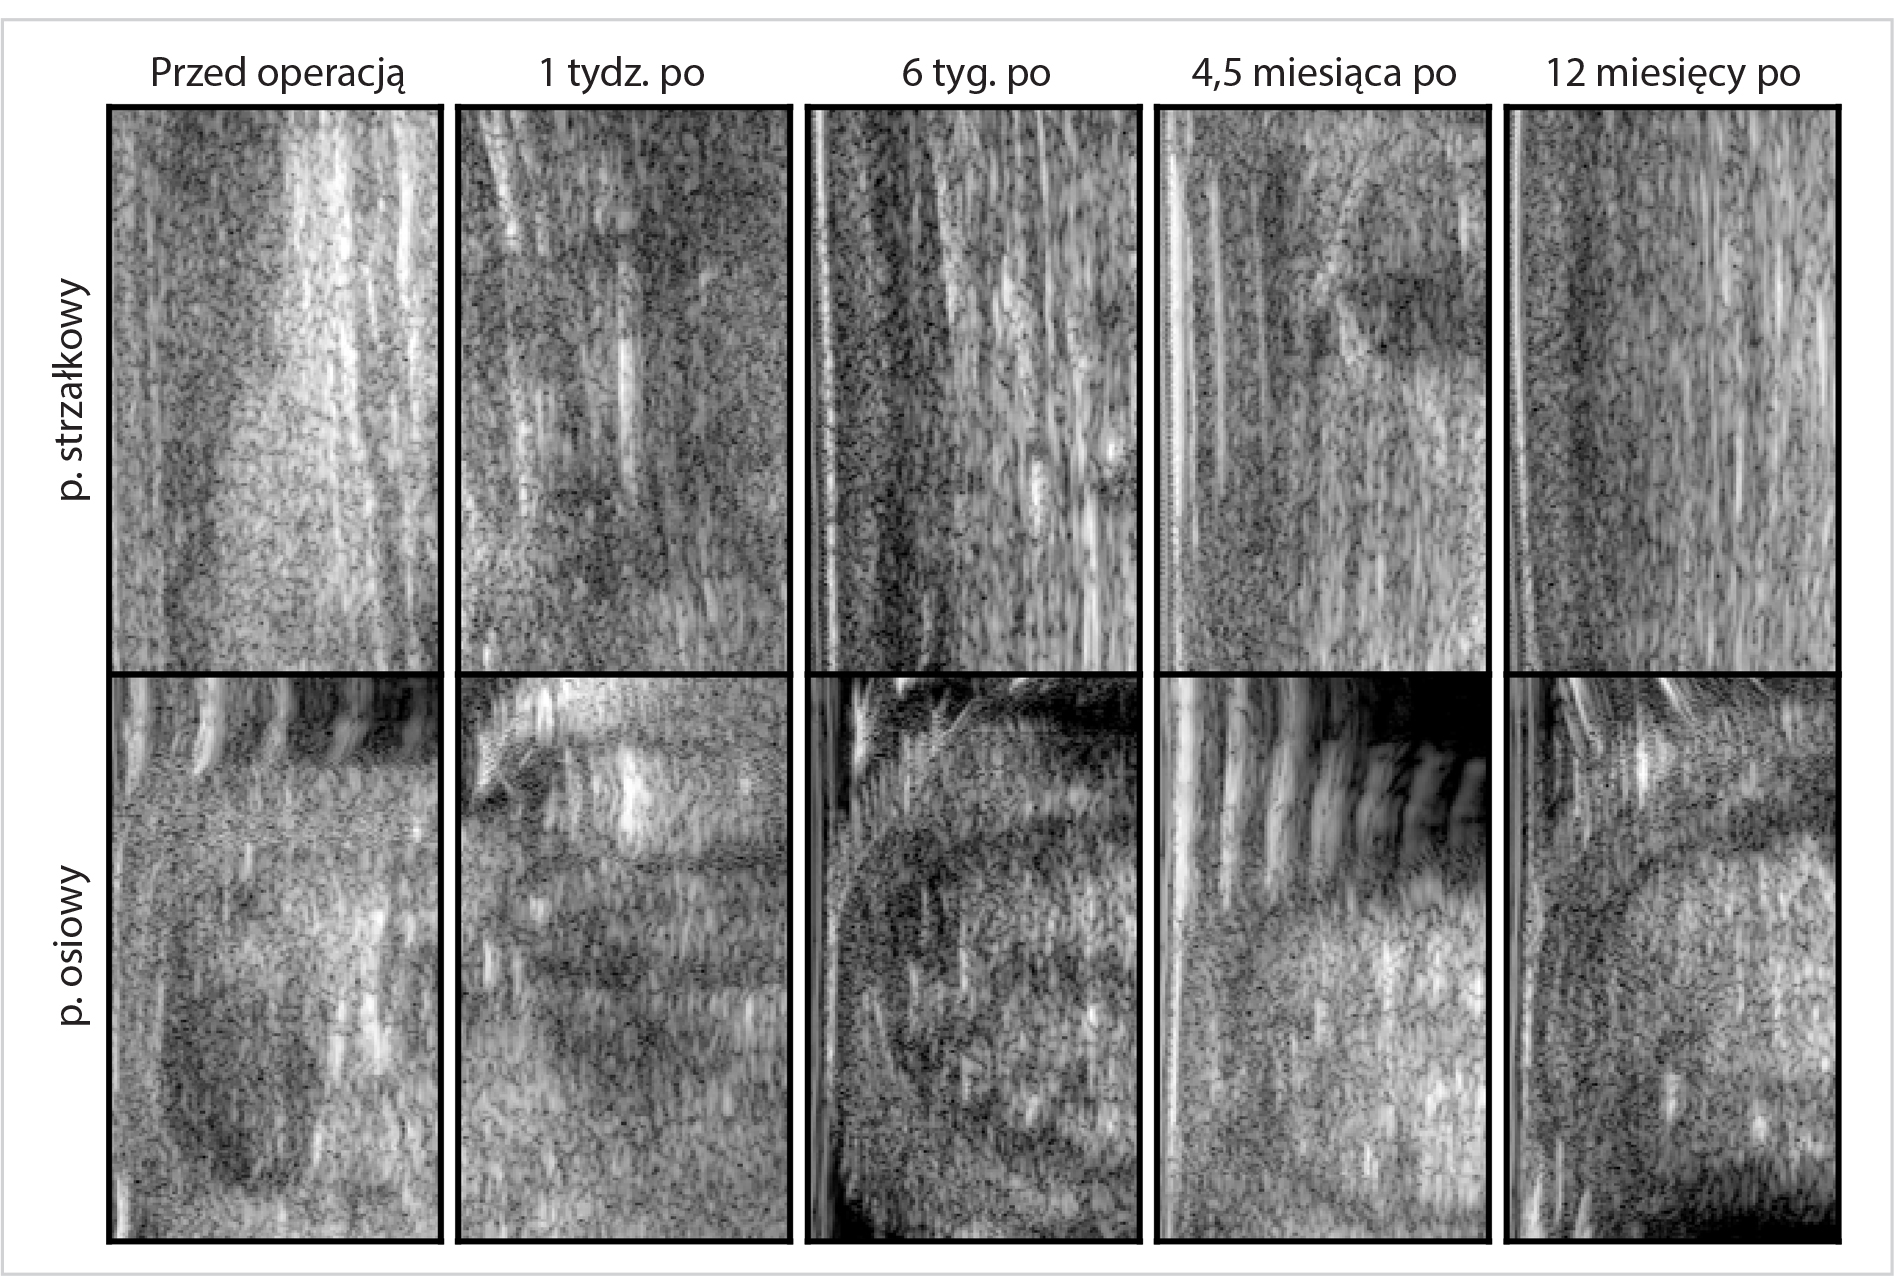
\includegraphics[width=\textwidth]{figures/Data_US_sample.jpg}
	\caption{Wizualizacja przykładowych danych USG w kolejnych tygodniach po zszyciu ścięgna w przekrojach osiowych i strzałkowych.}
	\label{fig:US_sample}
\end{figure}
W ogólności można zaobserwować ułożenie włókien ścięgnistych na przekrojach strzałkowych i teksturę oraz tkanki otaczające ścięgno na przekrojach osiowych. Jednak szczegółowa analiza załączonych obrazów może być wykonana jedynie przez specjalistę radiologa. 

Utrudniona w stosunku do obrazów RM interpretacja USG ma związek z obecnymi artefaktami w USG i z szumem ziarnistym tworzącym losowe wzorce. Jakość obrazu obniża również jego wartość kliniczną, co wskazują analizy zamieszczone w tej pracy jak i w wielu pracach innych autorów (zob. np. \cite{Khan2003, Ibrahim2013}). Dlatego na początku zdecydowano się przeprowadzić test polegający na prostym zadaniu klasyfikacji binarnej chory/zdrowy (podobnie jak dla badań RM zamieszczonych w Sekcji \ref{binaryMRI}). Ma to na celu porównanie możliwości interpretacji wnioskowania na podstawie obrazów RM i USG. Wyniki dla szkolenia z wykorzystaniem kroswalidacji z 4 segmentami zamieszczono w Tab. \ref{tab:usg-binary}.
\renewcommand{\arraystretch}{1.2}
\begin{table}[]
	\centering
	\scriptsize
	\setlength{\tabcolsep}{3pt}
	\setlength\extrarowheight{2pt}
	\caption{Wyniki szkolenia się sieci dla problemu binarnego na zbiorze treningowym dla danych z USG. Pogrubieniem oznaczono najlepsze wyniki ACC.}
	\label{tab:usg-binary}
	\begin{tabular}{l||c|c|c||c|c|c}
		%\hline
		& \multicolumn{3}{c}{\textbf{p. strzałkowy}} & \multicolumn{3}{c}{\textbf{p. osiowy}} \\
		\textbf{Model} & \textbf{ACC} & \textbf{PPV} & \textbf{TPR} & \textbf{ACC} & \textbf{PPV} & \textbf{TPR} \\ \hline \hline
		AlexNet & 0,846$\pm$0,087 & 0,92$\pm$0,08 & 0,78$\pm$0,11 & 0,843$\pm$0,075 & 0,93$\pm$0,06 & 0,73$\pm$0,11  \\ \hline
		Inception-v3 & \textbf{0,916}$\pm$0,049 & 0,97$\pm$0,04 & 0,90$\pm$0,06 & 0,901$\pm$0,052 & 0,95$\pm$0,3 & 0,87$\pm$00,07 \\ \hline
		ResNet-50 & 0,907$\pm$0,039 & 0,96$\pm$0,05 & 0,89$\pm$0,08 & \textbf{0,912}$\pm$0,046 & 0,95$\pm$0,04 & 0,88$\pm$0,06 \\ 
	\end{tabular}
\end{table}
\renewcommand{\arraystretch}{1}

Wszystkie modele wyszkolono oddzielnie na przekrojach osiowych i oddzielnie na strzałkowych. Żeby zbalansować dane, przekroje od zdrowych ochotników powiększono poprzez odbicie, a przekroje od chorych pacjentów próbkowano. Dokładność dla najlepszego modelu w przekroju osiowym wyniosła 91,6\%, a w przekroju strzałkowym 91,2\%. Dla porównania, dokładność binarnej klasyfikacji na danych z RM wyniosła 99,83\%. Wyniki te potwierdzają możliwość lepszej interpretacji danych RM dla zadanego problemu, jednak nie dyskryminują USG. W celu polepszenia powyższych rezultatów eksperymentowano również z możliwością klasyfikacji binarnej z wykorzystaniem jedynie obszaru ROI, jednakże działania te przyniosły odwrotny skutek.  

Kolejnym krokiem eksperymentu było porównanie jakości oceny procesu gojenia. W badaniu wykorzystano ponownie paradygmat end-to-end i zmianę warstwy klasyfikującej na regresję z funkcją kosztu określoną jako średni błąd kwadratowy. Dla tej metody próbowano również odtworzyć schemat sprawdzony dla RM, bazujący na treningu binarnym oraz ekstrakcji i redukcji cech, jednak w przypadku USG otrzymane wyniki nie były na tyle satysfakcjonujące, aby zamieszczać je w tej pracy. Ostatecznie wyniki szkolenia sieci w paradygmacie end-to-end zamieszczono w Tab. \ref{tab:usg_train_cross-validation}.
\renewcommand{\arraystretch}{1.2}
\begin{table}[h]
	\scriptsize
	\setlength{\tabcolsep}{3pt}
	\centering
	\caption{Wyniki predykcji wzorca odniesienia dla pacjentów testowych, dla danych z USG. Pogrubieniem oznaczono najlepsze wyniki, osobno dla przekrojów osiowych i strzałkowych}
	\label{tab:usg_train_cross-validation}
	\begin{tabular}{lc||c|c|c|c|c|c}
		%\hline
		& & \multicolumn{6}{c}{\textbf{p. strzałkowy}} \\
		\textbf{Model} & & \textbf{SCT} & \textbf{TT} & \textbf{STE} & \textbf{TE} & \textbf{TU} & \textbf{TisE} \\ \hline \hline
		AlexNet & MAE & 0,96$\pm$0,41 & 0,80$\pm$0,27 & 0,82$\pm$0,29 & 0,95$\pm$0,41 & 0,87$\pm$0,39 & 1,08$\pm$0,47  \\
		& MAX-AE & 1,75 & 1,32 & 1,87 & 1,35 & 1,61 & 2,03 \\ 
		& Corr & 0,53 & 0,69 & 0,11 & \textbf{0,68} & 0,31 & 0,22 \\ \hline
		Inception-v3 & MAE & \textbf{0,88}$\pm$0,35 & \textbf{0,67}$\pm$0,23 & \textbf{0,80}$\pm$0,31 & 0,82$\pm$0,23 & \textbf{0,84}$\pm$0,32 & \textbf{0,93}$\pm$0,29  \\
		& MAX-AE & 1,69 & 1,32 & 1,69 & \textbf{1,31} & \textbf{1,58} & \textbf{1,64} \\ 
		& Corr & \textbf{0,83} & \textbf{0,71} & 0,19 & 0,64 & \textbf{0,56} & \textbf{0,71} \\ \hline
		ResNet-50 & MAE & 0,89$\pm$0,12 & 0,74$\pm$0,15 & 0,83$\pm$0,22 & \textbf{0,81}$\pm$0,31 & 0,92$\pm$0,31 & 0,99$\pm$0,32 \\
		& MAX-AE & \textbf{1,53} & \textbf{1,22} & \textbf{1,64} & 1,43 & 1,67 & 1,71 \\
		& Corr & 0,62 & 0,38 & \textbf{0,23} & 0,62 & 0,12 & 0,43 \\ \hline \hline
		& & \multicolumn{6}{c}{\textbf{p. osiowy}} \\
		
		AlexNet & MAE & \textbf{0,98}$\pm$0,39 & 0,83$\pm$0,33 & 0,82$\pm$0,35 & 0,94$\pm$0,52 & 0,95$\pm$0,50 & 0,86$\pm$0,28  \\
		& MAX-AE & \textbf{1,79} & \textbf{1,36} & 1,86 & 1,41 & 1,61 & 1,59 \\ 
		& Corr & 0,45 & 0,62 & 0,20 & 0,60 & 0,03 & 0,59 \\ \hline
		Inception-v3 & MAE & 1,03$\pm$0,46 & \textbf{0,70}$\pm$0,24 & \textbf{0,76}$\pm$0,26 & \textbf{0,86}$\pm$0,19 & 0,87$\pm$0,32 & \textbf{0,85}$\pm$0,25  \\
		& MAX-AE & 2,52 & \textbf{1,45} & \textbf{1,45} & \textbf{1,24} & 1,67 & \textbf{1,56} \\ 
		& Corr & \textbf{0,77} & \textbf{0,69} & \textbf{0,22} & \textbf{0,65} & \textbf{0,55} & \textbf{0,72} \\ \hline
		ResNet-50 & MAE & 1,05$\pm$0,31 & 0,78$\pm$0,33 & 0,80$\pm$0,24 & 1,02$\pm$0,25 & \textbf{0,87}$\pm$0,15 & 0,91$\pm$0,28 \\
		& MAX-AE & 1,98 & 1,51 & 1,59 & 1,63 & \textbf{1,45} & 1,57 \\
		& Corr & 0,52 & 0,47 & 0,21 & 0,64 & 0,18 & 0,57 \\ 
	\end{tabular}
\end{table}
\renewcommand{\arraystretch}{1}

Największą liczbę najlepszych rezultatów otrzymano odpowiednio dla sieci Inception-v3 i ResNet-50 dlatego te modele zostały dalej porównane z proponowaną metodą. W tym celu wyniki MAE, MAX-AE i Corr zostały wyliczone dla zbioru pacjentów testowych i zebrane w Tab. \ref{tab:USGvsRM-cross-validation}.

\renewcommand{\arraystretch}{1.2}
\begin{table}[h]
	\scriptsize
	\setlength{\tabcolsep}{1pt}
	\centering
	\caption{Porównanie wyników oceny automatycznej bazującej na danych USG i RM na zbiorze testowym. Pogrubieniem oznaczono najlepsze wyniki.}
	\label{tab:USGvsRM-cross-validation}
	\vspace{-0.5cm}
	\begin{tabular}{lc||c|c|c|c|c|c}
		%\hline
		& & \multicolumn{6}{c}{\textbf{p. strzałkowy}} \\
		\textbf{Model} & & \textbf{SCT} & \textbf{TT} & \textbf{STE} & \textbf{TE} & \textbf{TU} & \textbf{TisE} \\ \hline \hline
		Inception-v3 & MAE & \textbf{0,81}$\pm$0,38 & 0,63$\pm$0,06 & \textbf{0,56}$\pm$0,18 & 0,85$\pm$0,20 & 0,54$\pm$0,04 & 0,87$\pm$0,29 \\
		& MAX-AE & 1,59 & 1,79 & 1,7 & \textbf{1,25} & \textbf{1,38} & 1,69 \\
		& Corr & 0,80 & 0,77 & 0,31 & 0,52 & \textbf{0,69} & 0,62 \\ \hline
		ResNet-50 & MAE & 0,88$\pm$0,33 & 0,65$\pm$0,15 & 0,66$\pm$0,09 & 0,83$\pm$0,25 & 0,75$\pm$0,12 & 0,93$\pm$0,22 \\
		& MAX-AE & \textbf{1,49} & \textbf{1,26} & 1,74 & 1,48 & 1,78 & 1,71 \\
		& Corr & 0,60 & 0,55 & 0,25 & 0,55 & 0,34 & 0,56 \\
		\hline \hline
		& & \multicolumn{6}{c}{\textbf{p. osiowy}} \\
		
		Inception-v3 & MAE & 0,84$\pm$0,54 & 0,75$\pm$1,45 & 0,58$\pm$0,10 & 0,83$\pm$0,10 & \textbf{0,53}$\pm$0,16 & \textbf{0,83}$\pm$0,30 \\
		& MAX-AE & 2,8 & 1,46 & \textbf{1,51} & 1,27 & 1,63 & 1,65 \\
		& Corr & 0,69 & 0,68 & 0,45 & 0,51 & 0,66 & 0,68 \\ \hline
		ResNet-50 & MAE & 0,92$\pm$0,37 & 0,76$\pm$0,32 & 0,68$\pm$0,08 & \textbf{0,81}$\pm$0,17 & 0,65$\pm$0,20 & 0,94$\pm$0,11 \\
		& MAX-AE & 2,01 & 1,56 & 1,61 & 1,69& 1,43 & \textbf{1,58}\\
		& Corr & 0,55 & 0,57 & \textbf{0,35} & 0,44 & 0,39 & 0,61 \\ \hline \hline
		& & \multicolumn{6}{c}{\textbf{Rezonans magnetyczny}} \\
		
		SVR & MAE & $1,05\pm0,12$ & \textbf{0,56}$\pm0,06$ & $0,75\pm0,08$ & $0,91\pm0,10$ & $0,91\pm0,09$ & $0,94\pm0,10$\\
		& MAX-AE & 2,62 & 1,82 & 1,92 & 2,54 & 2,01 & 2,38 \\
		& Corr   & \textbf{0,85} & \textbf{0,85} & 0,31 & \textbf{0,72} & 0,65 & \textbf{0,80} \\
		 
	\end{tabular}
\end{table}
\renewcommand{\arraystretch}{1}

Sieć, uzyskująca najlepsze rezultaty, wytrenowana na USG tj. Inception-v3, uzyskała wartości MAE w zakresie $0,53$ do $0,87$ i uśrednioną korelację Z-Fisher od $0,31$ do $0,8$.
Metoda oparta o USG charakteryzuje się lepszymi rezultatami Corr tylko dla parametrów STE i TU, czyli dla parametrów ocenianych przez wzgląd na krawędzie i na oś w płaszczyźnie strzałkowej. W przypadku miary MAE, metoda RM uzyskuje lepszy rezultat w parametrze TT, gdzie znaczący wpływ na ocenę maja cechy z ROI.

Bazując na powyższych rezultatach można wnioskować, że metoda oparta o dane USG może być komplementarna z proponowaną oceną bazującą na danych z RM. Zwłaszcza w kontekście oceny parametru TU jak i zmniejszenia błędu MAE w poszczególnych parametrach. Do tego celu potrzebna jest jednak dokładna analiza i zrozumienie podstaw wnioskowania sieci opartej o USG, a następnie wybór oraz realizacja odpowiedniej metody fuzji.

\section{Porównanie z metodą opartą o badania biomechaniczne}
\label{seq:comp-biomechanics}
W tej sekcji opracowana metoda została porównana z wynikami badań biomechanicznych i wynikami funkcjonalnego testu ATRS. Badania te były realizowane w ramach protokołu monitorowania rehabilitacji pacjentów opracowanego w klinice Carolina Medical Center (zob. Sekcja \ref{biomechanika}). 

W ramach projektu START możliwe było zebranie danych dla 30 spośród 60 pacjentów. Dane zawierały wyniki pomiaru zrealizowanego w dwóch krokach czasowych tj. w 26 i 52 tygodniu. Po wstępnych analizach, do porównań w tej pracy wykorzystano zebrane wyniki ATRS i deficyty sił mięśniowych będące rezultatem badań biomechanicznych. Dokładniej, określono 16 takich deficytów oznaczonych dalej w tej pracy $d1$--$d16$. W czterech pozycjach tj. kolano zgięte i wyprostowane oraz staw skokowy zgięty wyprostowany zrealizowano pomiary w warunkach izometrii i izokinetyki w trzech prędkościach kątowych 60$^\circ$/s, 120$^\circ$/s oraz 180$^\circ$/s  

Z uwagi na dużą liczbę pomiarów, w pierwszej kolejność zdecydowano się na przeprowadzenie analizy czynników głównych i identyfikację nowych zmiennych wyjaśniających w największym stopniu wariancję w zebranym zbiorze danych. Wyniki podsumowano w Tabeli \ref{tab:pca-muscles}.

\begin{table}[h]
	\centering
	\setlength{\tabcolsep}{3pt}
	\setlength\extrarowheight{2pt}
	\caption{Wyniki analizy czynników głównych dla 16-tu pomiarów deficytów mięśniowych w warunkach izometrii i izokinetyki. Oznaczono ładunki większe niż 0,7.}
	\label{tab:pca-muscles}
	\begin{tabular}{c|c|c|c|c}
		%\hline

		Zmienna&Czynnik1&Czynnik2&Czynnik3&Czynnik4 \\
		\hline \hline
		d1&\textbf{-0,77}&0,16&-0,04&-0,25 \\
		\hline
		d2&0,32&\textbf{-0,74}&0,038&-0,044 \\
		\hline
		d3&\textbf{-0,81}&0,26&-0,17&-0,24 \\
		\hline
		d4&0,09&-0,62&-0,50&-0,38 \\
		\hline
		d5&\textbf{-0,82}&0,13&-0,03&0,21 \\
		\hline
		d6&0,31&-0,53&-0,53&0,42 \\
		\hline
		d7&-0,67&-0,20&-0,34&-0,11 \\
		\hline
		d8&-0,12&-0,34&-0,67&0,43 \\
		\hline
		d9&-0,61&-0,01&-0,28&-0,36 \\
		\hline
		d10&0,07&\textbf{-0,84}&0,26&0,02 \\
		\hline
		d11&\textbf{-0,81}&-0,14&0,01&0,08 \\
		\hline
		d12&-0,11&\textbf{-0,93}&-0,01&-0,01 \\
		\hline
		d13&\textbf{-0,72}&-0,24&0,28&0,36 \\
		\hline
		d14&-0,12&\textbf{-0,81}&0,33&-0,25 \\
		\hline
		d15&-0,58&-0,32&0,39&0,53 \\
		\hline
		d16&-0,17&-0,62&0,23&-0,36 \\
		\hline\hline
		Udział&0,28&0,27&0,10&0,09 \\

	\end{tabular}
\end{table}

Z czterech czynników, 2 mają wyraźnie większy udział w wyjaśnianej wariancji, osiągając odpowiednio poziomy 28 i 27\%. Istotne jest również, że 3 z pięciu znaczących ładunków czynnikowych ($d1$, $d3$, $d5$) dla pierwszego czynnika znajdują się w przedziale $d1$--$d8$, które skojarzone są z pozycją kolana prostego oraz, że dla drugiego czynnika głównego sytuacja jest odwrotna i 3 z czterech ładunków czynnikowych ($d10$, $d12$, $d14$) znajdują się w przedziale $d9$--$d16$, czyli badania przy kolanie zgiętym. 

Co oczywiste, pozycja kolana wpływa znacząco na wynik badania biomechanicznego, dlatego w ramach dalszej pracy zdecydowano się na  analizę czynnikową dla wyprostowanego i zgiętego kolana oddzielnie. Wyniki zostały przedstawione w Tabeli \ref{tab:pca-muscles-knee-strait-bended}. 

\begin{table}[h]
	\centering
	\setlength{\tabcolsep}{3pt}
	\setlength\extrarowheight{2pt}
	\caption{Wyniki analizy czynników głównych dla 16-tu pomiarów deficytów mięśniowych, oddzielnie dla pozycji kolana zgiętego i wyprostowanego. Oznaczono ładunki większe niż 0,7.}
	\label{tab:pca-muscles-knee-strait-bended}
	\begin{tabular}{c|c|c||c|c|c}
		%\hline
		
		Zmienna&Czynnik1&Czynnik2&Zmienna&Czynnik1&Czynnik2 \\
		\hline \hline
		d1&\textbf{-0,82}&-0,14&d9&-0,26&0,64 \\
		\hline
		d2&-0,60&-0,37&d10&\textbf{-0,72}&-0,47 \\
		\hline
		d3&\textbf{0,88}&-0,20&d11&-0,52&\textbf{0,73} \\
		\hline
		d4&-0,36&-0,65&d12&\textbf{-0,83}&-0,34 \\
		\hline
		d5&\textbf{0,83}&-0,26&d13&-0,65&0,64 \\
		\hline
		d6&-0,57&-0,64&d14&\textbf{-0,81}&-0,43 \\
		\hline
		d7&0,55&-0,60&d15&-0,67&0,40 \\
		\hline
		d8&-0,03&\textbf{-0,80}&d16&-0,65&-0,38 \\
		\hline\hline
		Udział&0,41&0,26&&0,44&0,27 \\
		
	\end{tabular}
\end{table}

Ponownie można zaobserwować charakterystyczne rozróżnienie, kiedy to pierwszy czynnik główny dla badania w pozycji kolana wyprostowanego zawiera ładunki znaczące o nieparzystych numerach, a drugi czynnik posiada znaczące ładunki o parzystych numerach. W przypadku badania w pozycji kolana zgiętego sytuacja jest odwrotna i analogicznie można zaobserwować rozróżnienie. W tym przypadku podział wynika z pozycji stawu skokowego. Ładunki o nieparzystych numerach posiadają czynniki związane z badaniami w zgięciu stawu skokowego, a o parzystych w wyproście. Z uwagi na ten fakt do kolejnych porównań zostały zdefiniowane następujące 4 zmienne:
\begin{enumerate}
	\item $ZZ$ -- wyniki dla pozycji kolano zgięte i staw skokowy zgięty.
	\item $ZW$ -- wyniki dla pozycji kolano zgięte i staw skokowy wyprost.
	\item $WZ$ -- wyniki dla pozycji kolano wyprostowane i staw skokowy zgięty.
	\item $WW$ -- wyniki dla pozycji kolano wyprostowane i staw skokowy wyprostowany.
\end{enumerate} 

Każda z nowo powstałych zmiennych składa się z czterech pomiarów: jednego dla izometrii i trzech dla izokinetyki. Dokładne zestawienie znajduje się w Tabeli \ref{tab:bio-new-factors}.

\begin{table}[h]
	\centering
	\setlength{\tabcolsep}{3pt}
	\setlength\extrarowheight{2pt}
	\caption{Komponenty i ich udział, wchodzące w skład nowych zmiennych opisujących biomechanikę.}
	\label{tab:bio-new-factors}
	\begin{tabular}{c|c|c|c|c||c}
		Zmienna&Czynnik1&Czynnik2&Czynnik3&Czynnik4&Udział \\
		\hline \hline
		ZZ&d9 (-0,61)&d11 (-0,88)&d13 (-0,92)&d15 (-0,77)&0,65\\
		\hline
		ZW&d10 (-0,86)&d12 (-0,91)&d14 (-0,92)&d16 (-0,77)&0,75\\
		\hline
		WZ&d1 (-0,85)&d3 (-0,90)&d5 (-0,87)&d7 (-0,72)&0,70\\
		\hline
		WW&d2 (-0,64)&d4 (-0,76)&d6 (-0,88)&d8 (-0,66)&0,55\\
		
			
	\end{tabular}
\end{table}

Taki podział wydaje się być intuicyjny, ale fakt otrzymania powyższych wyników w analizie numerycznej jest wartością dodaną potwierdzającą spójność danych i jakość przeprowadzonych badań przez fizjoterapeutów z Carolina Medical Center. 

W celu efektywnego porównania nowych zmiennych opisujących biomechanikę ścięgna i wyniku ATRS z predykcjami automatycznej metody oraz oceną radiologa, zdecydowano się dla badań radiologicznych przeprowadzić również analizę czynnikową. W obu przypadkach tj. oceny automatycznej i radiologa uzyskano minimalny udział w wyjaśnianej wariancji czynników innych niż pierwszy. Stąd możliwość wprowadzenia nowej zmiennej tj. czynnika1 zamiast 6 parametrów: $SCT$, $STE$, $TE$, $TisE$, $TT$, $TU$. Szczegółowe wyniki znajdują się w Tabeli \ref{tab:pca-gt-pred}.

\begin{table}[h]
	\centering
	\setlength{\tabcolsep}{3pt}
	\setlength\extrarowheight{2pt}
	\caption{Rezultaty analizy czynników głównych dla oceny radiologicznej i oceny automatycznej realizowanych z wykorzystaniem 6-ścio parametrycznej ankiety. Oznaczono ładunki większe niż 0,7.}
	\label{tab:pca-gt-pred}
	\begin{tabular}{c|c|c}
		Zmienna&Czynnik1 - ocena radiologa&Czynnik1 - ocena automatyczna \\
		\hline \hline
		SCT&\textbf{-0,79}&\textbf{-0,95}\\
		\hline
		STE&0,57&\textbf{0,86}\\
		\hline
		TE&\textbf{-0,85}&\textbf{-0,94}\\
		\hline
		TisE&\textbf{-0,71}&\textbf{-0,89}\\
		\hline
		TT&\textbf{-0,76}&\textbf{-0,72}\\
		\hline
		TU&\textbf{-0,88}&\textbf{-0,94}\\
		\hline \hline	
		Udział&0,57&0,78\\
			
	\end{tabular}
\end{table}

Można zaobserwować, że udział wyjaśnianej wariancji w pierwszym czynniku jest większy dla oceny automatycznej niż dla oceny radiologa. Subiektywna ocena eksperta wprowadza nieuniknioną niepewność do pomiaru, stąd wyniki generowane przez człowieka są w większym stopniu losowe niż wyniki oceny automatycznej. 

W kolejnych badaniach zestawione zostały interkorelacje nowych zmiennych. Na początku, w Tabeli \ref{tab:gtVSpred}, przedstawiono korelację oceny automatycznej z oceną radiologa.


\begin{table}[h]
	\centering
	\setlength{\tabcolsep}{3pt}
	\setlength\extrarowheight{2pt}
	\caption{Korelacja między oceną radiologa, a ocena automatyczną. Oznaczone wsp. korelacji są istotne z $p$ $<$ 0,05 dla $N$=30.}
	\label{tab:gtVSpred}
	\begin{tabular}{c|c|c}
		&Ocena automatyczna &Ocena radiologa \\
		\hline \hline
		Ocena automatyczna&1,0000&\textbf{0,8070}\\
		\hline
		Ocena radiologa&\textbf{0,8070}&1,0000\\
			
	\end{tabular}
\end{table}

Naturalnie, nowa zmienna opisująca ocenę radiologa koreluje z nową zmienną opisującą ocenę automatyczną. Fakt ten jest kolejnym potwierdzeniem na silny związek między zastosowanymi metodami przetwarzania obrazów i eksperckimi, ludzkimi spostrzeżeniami. 

W kolejnej Tabeli (tj. Tabeli \ref{tab:bioVSatrs}) przedstawiono wyniki korelacji nowych zmiennych opisujących biomechanikę z wynikami testu ATRS. 

\begin{table}[h]
	\centering
	\setlength{\tabcolsep}{3pt}
	\setlength\extrarowheight{2pt}
	\caption{Korelacja badań biomechanicznych z testem ATRS. Oznaczone wsp. korelacji są istotne z $p$ $<$ 0,05 dla $N$=30.}
	\label{tab:bioVSatrs}
	\begin{tabular}{c|c|c|c|c|c}
		&WW&WZ&ZW&ZZ&ATRS \\
		\hline \hline
		WW&1,0000&-0,2037&\textbf{0,4948}&-0,0436&-0,2190\\
		\hline
		WZ&-0,2037&1,0000&-0,0143&\textbf{0,5815}&0,1070\\
		\hline
		ZW&\textbf{0,4948}&-0,0143&1,0000&0,2324&-0,2620\\
		\hline
		ZZ&-0,0436&\textbf{0,5815}&0,2324&1,0000&0,1437\\
		\hline
		ATRS&-0,2190&0,1070&-0,2620&0,1437&1,0000\\
		
		
	\end{tabular}
\end{table}

Można zaobserwować istotną korelację pomiarów wykonanych przy takim samym ustawieniu kolana. Jest to istotniejsze nawet od ustawienia stawu skokowego. Z kolei analizując rezultaty korelacji z ATRS, można zaobserwować słabą korelację z wynikami pomiarów biomechanicznych. Uzasadnione jest zatem realizowanie w praktyce obydwu tych badań w celu skutecznego monitorowania rehabilitacji pacjentów.

W finalnym badaniu, w tej sekcji zestawiono nowe zmienne opisujące ocenę radiologa i ocenę automatyczną, z wynikami badań biomechanicznych i ATRS. Szczegółowe rezultaty przedstawiono w Tabeli \ref{tab:bioATRSvspredGT}.

\begin{table}[h]
	\centering
	\setlength{\tabcolsep}{3pt}
	\setlength\extrarowheight{2pt}
	\caption{Korelacja badań biomechanicznych i testu ATRS z badaniami radiologicznymi ocenionymi automatycznie i przez radiologa. Oznaczone wsp. korelacji są istotne z $p$ $<$ 0,05 dla $N$=30.}
	\label{tab:bioATRSvspredGT}
	\begin{tabular}{c|c|c}
		&ocena automatyczna&ocena radiologa \\
		\hline \hline
		WW&0,1197&0,0706\\
		\hline
		WZ&0,1576&0,1931\\
		\hline
		ZW&0,3429&0,3092\\
		\hline
		ZZ&0,3100&0,2996\\
		\hline
		ATRS&\textbf{0,3854}&0,2088\\
		
	
	\end{tabular}
\end{table}

Można zaobserwować, że wskazania radiologa słabo korelują z wynikami badań biomechanicznych oraz ATRS, co jest zgodne z praktyką kliniczną -- dlatego zalecane jest wykonywanie badań radiologicznych, które dostarczając komplementarnych informacji.

Interesującym rezultatem jest wynik istotnej, niewielkiej korelacji oceny automatycznej z ATRS. Można wnioskować, że eliminacja losowości wynikającej z czynnika ludzkiego, spowodowała usystematyzowanie oceny, a jednocześnie uwspulnienie pewnych informacji, które obecne są również w ustrukturyzowanym teście ATRS. Wynik ten wyznacza ciekawy kierunek dalszych prac, celem odnalezienia informacji wspólnych i stworzenia komplementarnego testu maksymalizującego informację dla lekarza prowadzącego przy jednoczesnej minimalizacji objętości protokołu monitorowania pacjentów.

\chapter{Podsumowanie}

W ramach pracy udało się osiągnąć wszystkie postawione cele. Cel główny tj. opracowanie automatycznej metody oceny gojenia się ścięgna Achillesa został osiągnięty poprzez zastosowanie unikalnej fuzji cech wyuczonych przez model głębokiej sieci neuronowej i cech wyekstrahowanych z wykorzystaniem klasycznych metod przetwarzania obrazów. Wnioski zostały spisane w Rozdziale \ref{NewMethod} podzielonym na trzy sekcje. W pierwszej przedstawiono szczegółowy opis komponentów oraz ich parametrów wraz z unikalnymi w skali światowej danymi. W drugiej, zaprezentowano wyniki eksperymentów mających na celu dobór komponentów i ich parametrów oraz optymalizacji czasu, jakości i kosztów związanych z zastosowaniem nowej metody. W ostatniej, trzeciej sekcji zaprezentowano szczegółową walidację wraz z analizą rozbieżności między nowym podejściem, a oceną radiologa.

W toku prac, zrealizowano również wszystkie cztery cele szczegółowe. Pierwszy, tj. "wybór efektywnego kosztowo i czasowo protokołu badania bazującego na technikach obrazowania medycznego, a dokładniej Rezonansu Magnetycznego" zrealizowano poprzez badania zamieszczone w p. \ref{seq:protocol_selection}. Najważniejszym rezultatem tych prac jest określenie utylitarnego protokołu składającego się tylko z jednej, trwającej jedynie 5 min. sekwencji RM. 

Drugi cel, tj. "przetestowanie różnego rodzaju podejść związanych ze szkoleniem głębokich sieci neuronowych" zrealizowano poprzez zestawienie wyników działania nowej metody z wynikami alternatywnego podejścia tj. szkolenia sieci w oparciu o paradygmat end-to-end (zob. p. \ref{seq:end-to-end}). W zestawieniu z alternatywną metodą analizy obrazów RM, wykazano przewagę zaproponowanego podejścia, a dokładniej uzyskano lepsze rezultaty korelacji w każdym z sześciu ocenianych parametrów oraz dla czterech z nich, niższy absolutny błąd średni.

Kolejny cel, tj. "Porównanie wyników oceny nowej metody z wynikami klasyfikacji bazującej na danych z ultrasonografii" zrealizowano dołączając do pracy wyniki automatycznej interpretacji obrazów USG (zob. p. \ref{seq:comp-usg}). W szczególności wykazano możliwość synergii obu podejść, bazując na większej izotropowości danych USG i dobrych wyników oceny parametrów widocznych w płaszczyźnie strzałkowej.

Finalnie, ostatni cel, tj. "porównanie wyników oceny nowej metody z oceną funkcjonalną, rutynowo stosowana do wspomagania rehabilitacji po urazie ścięgna" osiągnięto uzyskując unikalne dane pomiarów biomechanicznych i testu ATRS, a następnie zestawiając je z wynikami nowo-opracowanej metody (zob. \ref{seq:comp-biomechanics}). Pokazano przydatność wykonywania badań radiologicznych, przez wzgląd na odmienność niesionej informacji, jednocześnie określono potencjalny obszar optymalizacji w zakresie niewielkiej, ale istotnej korelacji z wynikami testu ATRS.  

W ramach powyższych prac nad nowym podejściem do oceny procesu gojenia się ścięgna Achillesa w badaniach RM, całość zadań dotyczących głębokich sieci neuronowych została zrealizowana przez autora tej pracy. Pełnił on również rolę głównego badacza, projektując i współrealizując prace nad fuzją cech (w szczególności w ramach testów perceptronu wielowarstwowego i SVR jako typów meta-regresji). Autor tej pracy nadzorował również i planował eksperymenty grupy tworzącej metody bazujące na paradygmacie end-to-end oraz wykorzystywane do interpretacji obrazów USG, a następnie samodzielnie dokonał ich porównania z proponowanym w tej pracy podejściem. 

Wszystkie wyniki mają charakter innowacyjny. Nie istnieje obecnie wedle najlepszej wiedzy autora tej pracy alternatywne podejście do usystematyzowanej i wyliczanej automatycznie oceny stanu gojenia się ścięgna Achillesa widocznego w badaniach RM. Rozprawa ta stanowi zatem kompleksowy opis obecnego \textit{state-of-the-art} dla przedmiotowego problemu. Biorąc pod uwagę, że w przedstawionym stanie wyniki oceny automatycznej korelują z oceną radiologa nawet na poziomie 0,85, a minimalny uzyskany absolutny błąd średni równy jest 0,56, krytyczne w opinii autora tej pracy staje się polepszenie wzorca odniesienia. W dalszym toku prac planowana jest zatem stała współpraca m.in. z radiologami celem realizacji ocen przez kolejnych specjalistów oraz wielo-ośrodkowe zbieranie nowych wolumenów danych. Planowane jest również przeprowadzenie badań w zakresie usprawnienia przetwarzania danych, w szczególności w kwestii automatycznej segmentacji ROI. Finalnie, praca ta stanowi również fundament pod rozpoczęcie nowych testów dotyczących pokrewnych zadań jak ocena gojenia się podobnych struktur typu więzadeł stawu kolanowego, skokowego, barkowego, czy łokciowego. Polepszenie skuteczności wspomagania rehabilitacji w obszarze układu mięśniowo-szkieletowego stanowi według autora tej pracy ciekawe wyzwanie badawcze, jak również ma wymiar praktyczny. Już teraz bowiem, według danych Krajowej Izby Fizjoterapeutów, po zwolnieniach z pracy dotyczących ciąży, zwolnienia na skutek dolegliwości mięśniowo-szkieletowych stanowią drugi powód absencji w pracy w Polsce.
%- jeden radiolog więc ankieta ok
%- AlexNet uczy się bardziej generycznych cech niż ResNet, który zwraca uwagę na szczególy: https://www.researchgate.net/post/Can_AlexNet_be_a_better_feature_extractor_than_ResNet

%https://icmlviz.github.io/icmlviz2016/assets/papers/4.pdf

%Wydzielenie stanu przed operacją i oznaczenie osobną etykietą w procesie treningu mogłoby doprowadzić do polepszenia rezultatu, co jest sugestią dla przyszłych prac związanych z rozwojem metody.

%TU - Polepszenie w zakresie oceny tego parametru może być uzyskane w przypadku zastosowania bardziej jednorodnych danych RM lub USG.

